\section{Documentos y Código}
\subsection{Documentación Técnica}

\href{https://github.com/dexaxi/RecursosSolarcore/blob/main/Assets/Documentation/Memoria%20-%20%C3%81ngel/tfg-template-master/EcoRescue.pdf}{Documentación}

\subsection{Repositorios}
\begin{itemize}
  \item DUJAL: \url{https://github.com/dexaxi/TFG_unity_package}
  \item UniTask: \url{https://github.com/Cysharp/UniTask}
\end{itemize}

\section{Tablas y figuras}

\subsection{Diagrama de Clases completo}

\begin{figure}[H]
  \centering
  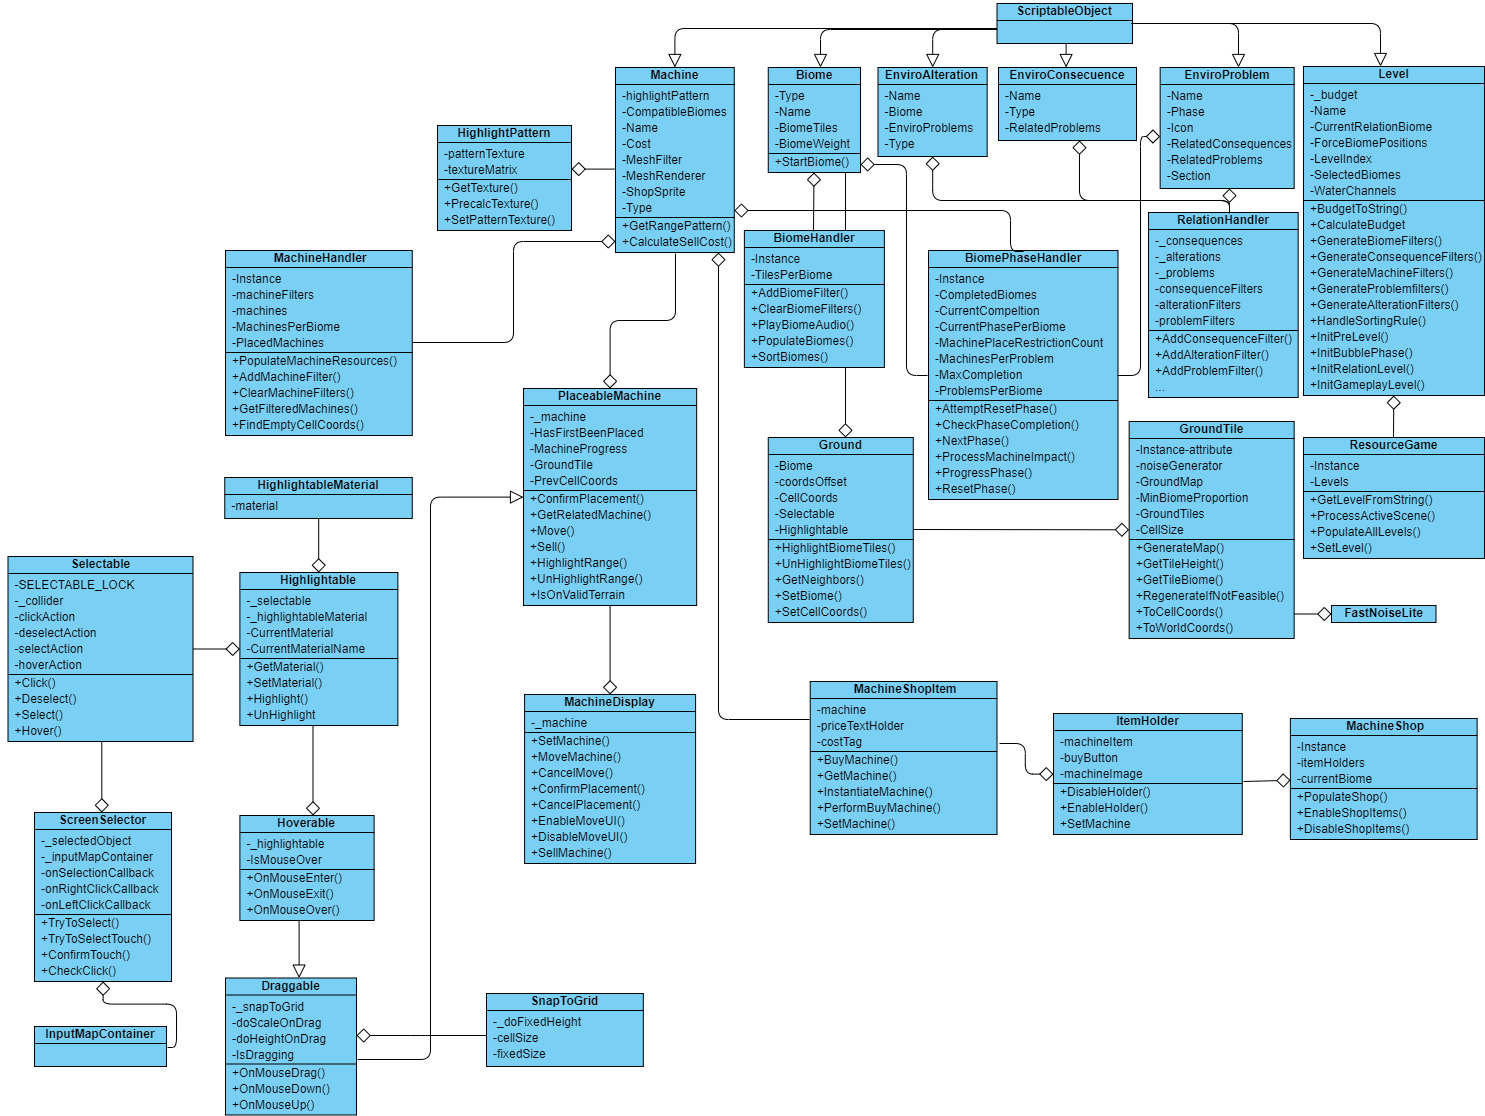
\includegraphics[width=450px,clip=true]{Logic_Class_Diagram.png}
  \caption{Diagrama de Clases completo}
  \label{fig:logicUML}
\end{figure}
\raggedbottom


\subsection{Resultados del Cuestionario}
% Insertar una figura
\begin{figure}[H]
  \centering
  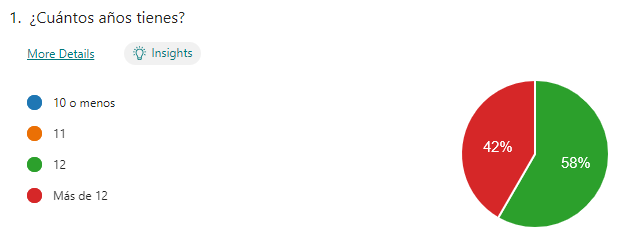
\includegraphics[width=450px,clip=true]{questionario_1.png}
  \caption{¿Cuántos años tienes?}
  \label{fig:questionario_1}
\end{figure}
\raggedbottom


% También con \pagebreak